%%% EtherPad for Discrete Mathematics VO
%%% http://www.informatik-forum.at/showthread.php?104454-Notes-2013WS-VO_01
%%% Past pads:
%%%     * 2013-10-17: committed by patrikf
%%%     * 2013-10-18: committed by patrikf
%%%     * 2013-10-24: committed by patrikf
%%%     * 2013-10-25: committed by patrikf
%%%     * 2013-11-08: committed by neroburner

% Discrete Mathematics Lecture Notes 2013-11-21

\section{Generating Functions}
\lecturedate[\baselineskip]{2013-11-21}

Generating functions provide a tool for coping with combinatorial enumeration problems. The ordinary generating function defines the sum of a sequence $a_n$:
\[
	(a_n)_{n≥0} = \sum_{n≥0} a_n z^n \text{, formal power series}
\]
\paragraph{Operations on generating functions:}
\begin{itemize}
	\item Two power series can be added:
	\[
		\sum_{n≥0} (a_n + b_n) z^n \text{,}
	\]

	\item multiplied:
	\[
		\sum_{n≥0}\sum_{k=0}^n a_k b_{n-k} z^n \qquad \text{(Cauchy product),}
	\]

	\item and if $b_0 ≠ 0$, we can also divide a power series by another power series:
	\[
	    \frac{
	        \sum a_n z^n
	    }{
	        \sum b_n z^n
	    } =
	        \sum c_n z^n
	\]
\end{itemize}

If we have
\[
    (*) = \sum_{n≥0} a_n z^n = \lim_{n \to ∞} \sum_{k=0}^{n} a_k z^k
\]

and $(*)$ is convergent, then the domain of convergence is a disk with center (0,0) and the radius of convergence is $R$:
\[
    R = \frac1{\overline{\lim} \sqrt[n]{|a_n|}} \in [0, \infty]
\]

\Theorem.
Let
\[
    f(z) = \sum a_n (z-z_0)^n,
    a_i\in \mathbb{C},
    R = \frac{1}{\overline{\lim} \sqrt[n]{|a_n|}}
\]
Then
\begin{enumerate}[a)]
	\item $|z - z_0| < R \implies f(z)$ absolutely convergent, i.e.
	      $\sum |a_n| (z-z_0)^n$ convergent

	\item $|z - z_0| > R \implies f(z)$ divergent
\end{enumerate}

\textbf{Examples.}
\begin{align*}
    &\sum_{n≥0} z^n =
        \frac1{1-z}\quad\text{for $|z|<1$, } R = 1 \\
    &\sum_{n≥0} \frac{z^n}{n!} =
        e^z, ~R = ∞ \\
    &\sum_{n≥0} n! z^n, ~R = 0
\end{align*}
Inside the disk of convergence, we even have \emph{uniform convergence} (allows interchange of limits).
\begin{align*}
    \frac1{(1-z)^2}
    &= \left(\frac1{1-z}\right)'
    = \left(\sum_{n>=0} z^n\right)'
    = \sum_{n≥1} n z^{n-1} \\
    \log\frac{1}{1-z} &= \sum_{n≥1} \frac{z^n}{n}
\end{align*}

\Theorem. (Identity theorem for power series).
Let
\[
    f(z) = \sum_{n≥0} a_n (z-z_0)^n,
    \text{f(z) convergent for $|z-z_0| < \epsilon$}
\].
The coefficients $a_n$ are unique and satisfy
\[
    a_n = \frac{f^{(n)}(z_0)}{n!}.
\]
$f(z)$ is the \emph{Taylor series}.

\textbf{Corollary.}
\[
    \sum a_n (z-z_0)^n =
    \sum b_n (z-z_0)^n
    \text{ for } |z-z_0| < \epsilon
    \implies
    a_n = b_n.
\]

Since $f(z)$ generates the sequence $(a_n)$ by continued differentiation and evaluation, we call $f(z)$ the \dt{generating function}. In particular,
\begin{align*}
\sum a_n z^n & \text{ ordinary generating function} \\
\sum a_n \frac{z^n}{n!} & \text{ exponential generating function.}
\end{align*}


\subsection{Operations On Generating Functions}

Let sequence $(a_n)_{n≥0}$ correspond to the generating function $\displaystyle{\sum_{n≥0} a_n z^n = A(z)}$ and $(b_n)_{n≥0}$ correspond to $B(z)$.

\begin{itemize}
\item Addition
\begin{align*}
    (\alpha a_n + \beta b_n)_{n≥0}
        &\leftrightarrow \alpha A(z) + \beta B(z)
        &&\forall \alpha, \beta \in \mathbb{C}
        \quad\text{(Linearity)}
\end{align*}
\item Multiplication
\begin{align*}
    \left(\sum_{k=0}^{n} a_k b_{n-k} \right)
        &\leftrightarrow A(z) B(z),
        \text{ in particular: }
        \left(\sum_{k=0}^n a_k\right)_{n≥0} \leftrightarrow \frac{1}{1-z} A(z)
\end{align*}

\Remark.
\begin{align*}
    \hat{A}(z) = \sum_{n \geq n} a_n \frac{z^n}{n!}, \\
    \hat{B}(z) = \sum_{n \geq n} b_n \frac{z^n}{n!}, \\
    \left(\sum_{k=0}^n \binom{n}{ k} a_k b_{n-k}\right)_{n \geq 0}
        \leftrightarrow \hat A(z)\hat B(z)
\end{align*}

\item $
    (a_n \gamma^n)_{n≥0}
        ↔ A(\gamma z) $
\item $ (a_{n-1})_{n≥1}↔ z A(z)$
\begin{align*}
        (a_{n+1})_{n≥0} ↔ \frac{A(z)-a_0}z,
        EGF: (a_{n+1})_{n≥0} ↔ \hat A'(z) \\
\end{align*}
\item $(n a_n)_{n≥0}↔ z A'(z)$

\end{itemize}

\textbf{Example.}
\[
    \sum_{n≥0} (-1)^n z^n
    = \frac{1}{1+z} \quad\text{for $|z| < 1$}.
\]

\textbf{Example.}
\[
    \sum_{n≥0} n z^n
    = \frac{z}{(1-z)^2}
    = z \left(\frac1{1-z}\right)'.
\]

\textbf{Example.}
\[
    \sum_{n≥0} \binom{\alpha}{n} z^n
    = (1+z)^\alpha
    \quad\forall\alpha\in\mathbb{C}
\]

\textbf{Example.}
\begin{align*}
    a_n &= \sum_{k≥0}^n k\\
    \sum_{n≥0} a_n z^n
    &= \sum_{n≥0}
        \left(\sum_{k=0}^n k\right) z^n
    = \sum_{n≥0} \left(\sum_{k=0}^n  k\cdot 1\right) z^n
        = \left( \sum_{n≥0} n z^n \right) \left( \sum_{n≥0} 1 \cdot z^n \right)\\
    &= \frac{z}{(1-z)^3}
    = \frac12 z \left(\frac{1}{1-z}\right)''
    = \frac z2 \sum_{n≥2} n(n-1) z^{n-2}\\
    &= \frac z2 \sum_{n≥0} n(n-1) z^{n-2}
    = \sum_{n≥0} \frac{(n+1)n}{2} z^n
    = \sum_{n≥0} {\binom{n+1}{2}} z^n
\end{align*}

\Lemma.
\begin{gather*}
    \sum_{n≥0} {\binom{n+k-1}{k-1}} z^n
    = \frac1{(1-z)^k} \\
    (1 + z)^\alpha = \sum {\binom{a}{n}} z^n \\
\end{gather*}

Sketch of proof:
\[
    {\binom{n+k-1} {k-1}} = \ldots = (-1)^k{\binom{-k}{n}}
\]


\subsection{Recurrence relations}

\textbf{Example.}
Consider the Towers of Hanoi problem with $n$ disks. How many steps do we need to move the disks?

\begin{figure}[htbp]
  \centering  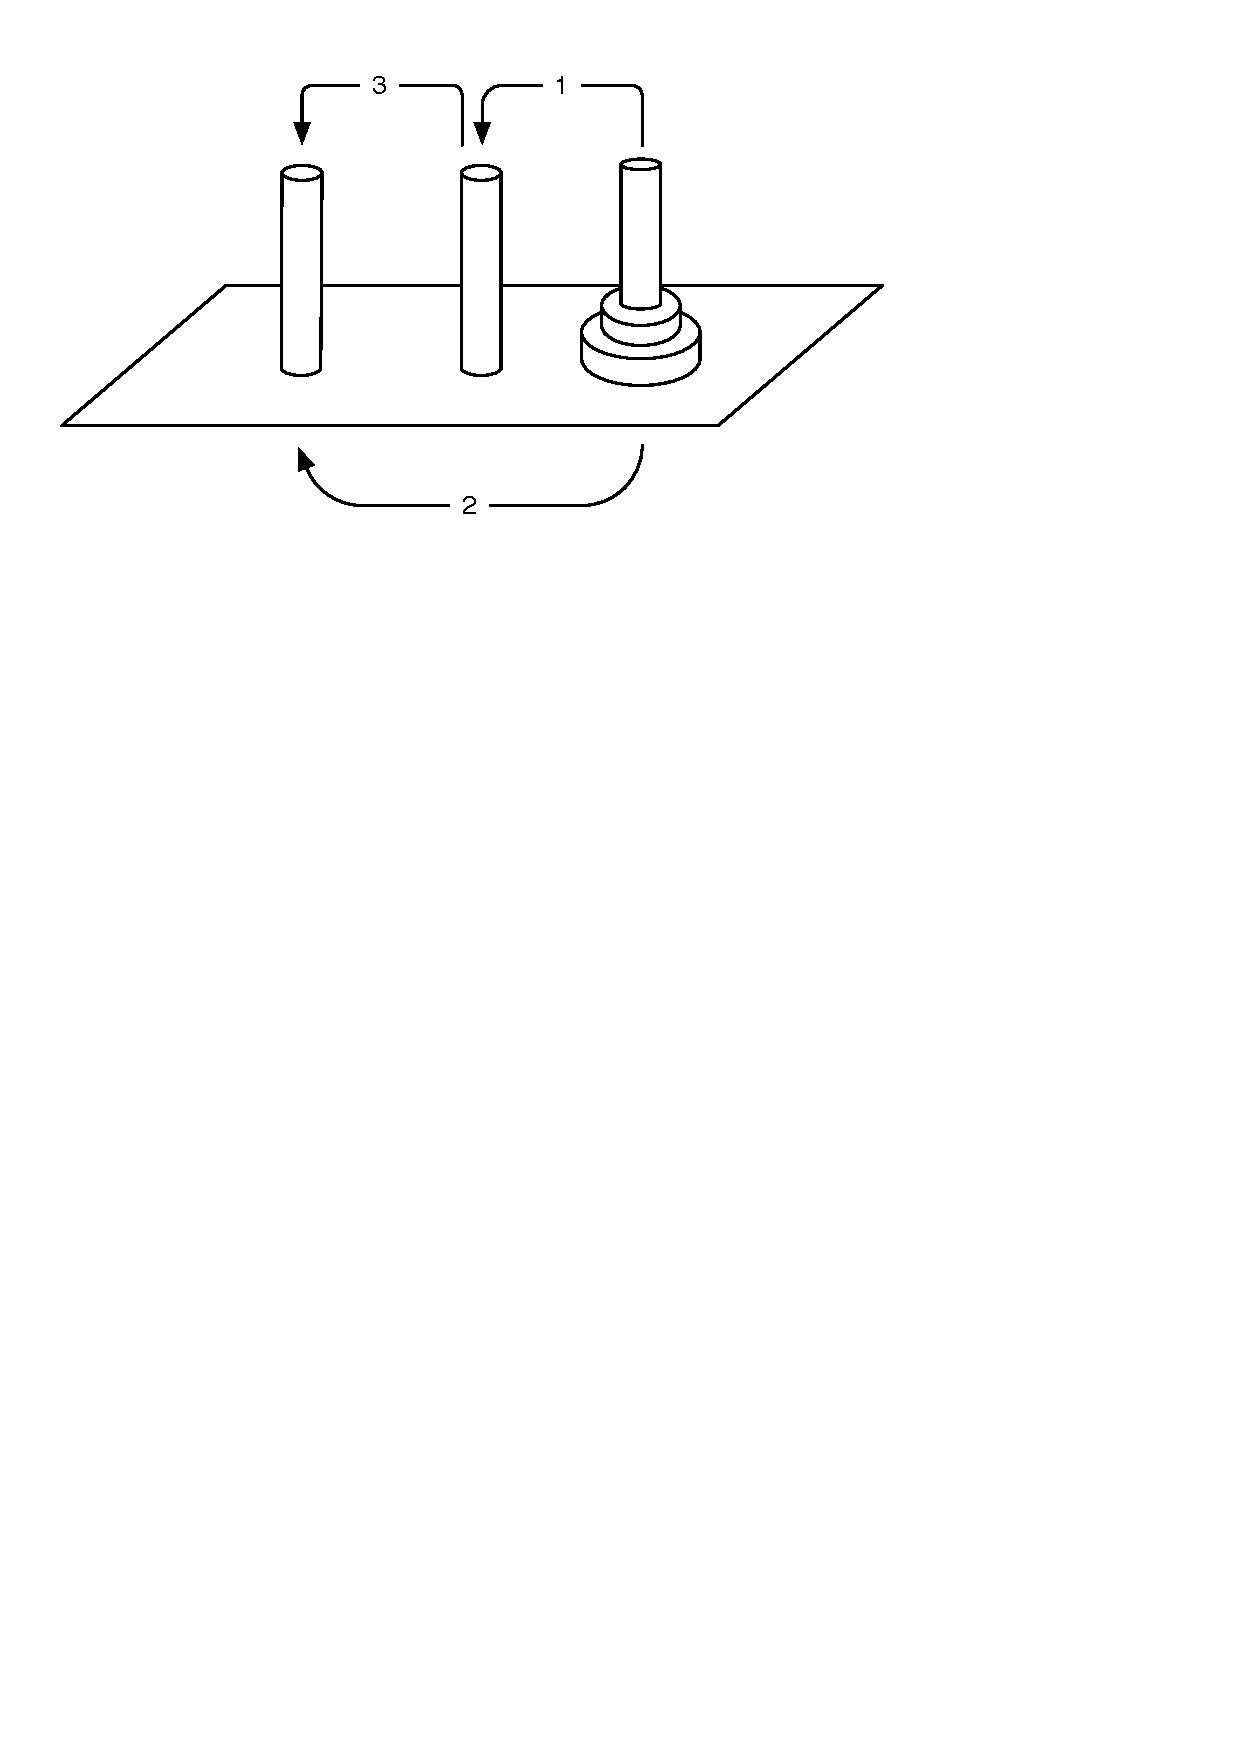
\includegraphics[width=0.8\textwidth]{02_higher_combinatorics/pics/TowerOfHanoi}
  \caption{Solution for the Tower of Hanoi with 2 disks}
\end{figure}
\begin{align*}
  a_0 = 0 \\
  a_1 = 1 \\
\end{align*}
For the $n+1$-th step, put $n$ disks to a temporary location, move the $n+1$-th disk, move the $n$ disks again.
\begin{align*}
  a_{n+1} &= 2 a_n + 1, a_n = 2^n - 1\\
  A(z) &= \sum_{n \geq 0} a_n z^n
\end{align*}

We multiply both sides with $z^{n+1}$ and sum up over $n$.

\begin{align*}
\sum_{n≥0} a_{n+1} z^{n+1} &= 2 \sum_{n \geq 0} a_n z^{n+1} + \sum_{n\geq 0} z^{n+1} \\
A(z) - \underbrace{a_0}_{0} &= 2z A(z) + \frac{z}{1-z}\\
A(z) &= 2 z A(z) + \frac{z}{1-z}\\
A(z) &= \frac{z}{(1-z)(1-2z)} \\
    &= \frac{\alpha}{1-z} + \frac{\beta} {1-2z}\\
    &= \frac{-1}{1-z} + \frac{1}{1-2z} \\
    &= -\sum_{n\geq 0} z^n + \sum_{n\geq 0} 2^n z^n\\
    &= \sum_{n\geq 0} (2^n-1) z^n\\
\end{align*}

\textbf{Example.}
\begin{align*}
    F_0 = 0, F_1 = 1, F_{n+2} = F_{n+1} + F_n \\
    F(z) &= \sum_{n≥0} F_n z^n : \\
    F(z) - \underbrace{F_0}_{0} - F_1 z &= z \left( F(z) - \underbrace{F_0}_{0} \right) + z^2 F(z)\\
    \implies F(z) &= \frac{z}{1-z-z^2} \\
    F(z) &= \frac{-z}{(z-z_1) (z-z_2)},
        \quad z_{1,2} = \frac{-1 \pm \sqrt{5}}{2} \\
    F(z) &= \frac1{\sqrt{5}} \cdot \frac{1}{1- \frac{1 + \sqrt{5}}{2} \cdot z} - \frac{1}{\sqrt{5}} \cdot \frac{1}{1- \frac{1 - \sqrt{5}}{2} \cdot z}  \\
    \implies F_n &= \frac{1}{\sqrt{5}}
		\left( \left( \frac{1+ \sqrt 5}{2} \right)^n
		- \left( \frac{1-\sqrt{5}}{2} \right)^n
		\right)
\end{align*}

In general:
\[
    a_{n+k} + q_1 a_{n+k-1} + \cdots + q_k a_n = 0
    \quad  \text{ (*) for }n \geq 0
\]
(*) is unique if the first $k$ elements are given

$a_0, ..., a_{k-1}$ given, $q_i$ are given constants

\begin{align*}
A(z) = \sum_{n\geq 0} a_n z^n
\end{align*}
\begin{align*}
\sum_{n\geq 0} a_{n+k} z^{n+k} + q_1 \sum_{n\geq 0}  a_{n+k-1}z^{n+k} + \ldots + q_k \sum_{n\geq 0} a_k z^{n+k} = 0
\end{align*}
\begin{align*}
A(z) - a_0 - a_1 z - \ldots - a_{k-1} z^{k-1} + q_1 z \left( A(z) - \sum_{i=0}^{k-2} a_i z^i \right) + \ldots + q_k z^k A(z) = 0\\
A(z) = \frac{ p(z) }{ 1 + q_1 z + q_2 z^2 + \ldots + q_k z^k } = \frac{p(z)}{q(z)} = \frac{p(z)}{\prod_{i=1}^{r} (z - z_i)^{\lambda_i}}
\end{align*}

Observation: $deg(p) < deg(q)$.

Use ansatz:
\begin{align*}
\frac{p(z)}{q(z)} &= \sum_{i=1}^{r} \sum_{j=1}^{\lambda_i} \frac{A_{ij}}{(z-z_i)^j} \\
&= \frac{A_{11}}{z-z_1} + \frac{A_{12}}{(z-z_1)^2} + \cdots + \frac{A_{1\lambda_i}}{(z-z_1)^{\lambda_i}} + \cdots \\
&= \sum_i\sum_j \frac{B_{ij}}{\left(1-\frac{z}{z_i}\right)^j}= \sum_i\sum_j B_{ij} \cdot \binom {n+j-1}{j-1} \cdot z_i^{-n}\\
&= \frac{\alpha}{1-z} + \frac{\beta}{1-2z} + \frac{\gamma}{(1-2z)^2} + \frac{\delta}{(1-2z)^3}\\
&\implies A_z = \sum_{n\geq 0}\left(p_1(n) \left( \frac{1}{z_1} \right)^n + p_2(n) \left( \frac{1}{z_2} \right)^n + \cdots + p_i(n) \left( \frac{1}{z_i} \right)^n \right)z^n \\
&deg(p_i) \leq \lambda_i + 1
\end{align*}
\TODO{Check the previous formulas for completeness}
\TODO{Complement with Patrik's notes}

\textbf{Example.}
\[
    a_{n+2} - 4 a_{n+1} - 4 a_n = 0 \quad n ≥ 0;  a_0, a_1 \text{ given}
\]
\[
    A(z) = \sum a_n z^n
\]
\begin{align*}
    A(z) - a_0 - a_1 z - 4z (A(z)-a_0) + 4z^2 A(z) &= 0 \\
    (1-4z + 4z^2) A(z) &= a_0 + a_1 z - 4a_0 z \\
    A(z) &= \frac{a_0 + (a1 - 4a_0)z}{1- 4z + 4z^2}\\
    &= \frac{a_0 + (a1 - 4a_0)z}{(1-2z)^2}\\
    &= \frac{C}{1-2z} + \frac{D}{(1-2z)^2} = (*)\\
    \implies a_0 + (a_1 - 4a_0)z &= C (1-2z) + D \\
    [z^0]: a_0 &= C+D \\
    [z^1]: a_1 - 4a_0 &= -2C \\
    \implies C, D
\end{align*}
\begin{align*}
    (*) = C \cdot \sum_n 2^n z^n + D \cdot \sum_n (n+1) \cdot 2^n z^n \\
    = \sum_n \left(2^n \cdot C + (n+1)\cdot 2^n D\right) z^n \\
    = \sum_n (a_n) z^n
\end{align*}

\TODO{Add inhomogeneous recurrence relation to above example, i.e., $0$ on the rhs of the initial equation is replaced by $f(n)$}

\subsection{Unlabeled Combinatorial Structures}

\textbf{Example.}
Binary tree (complete), (without cycles, plane, rooted, either no further children (external nodes, leaves) or 2 children (internal nodes))

\begin{figure}[htbp]
  \centering
    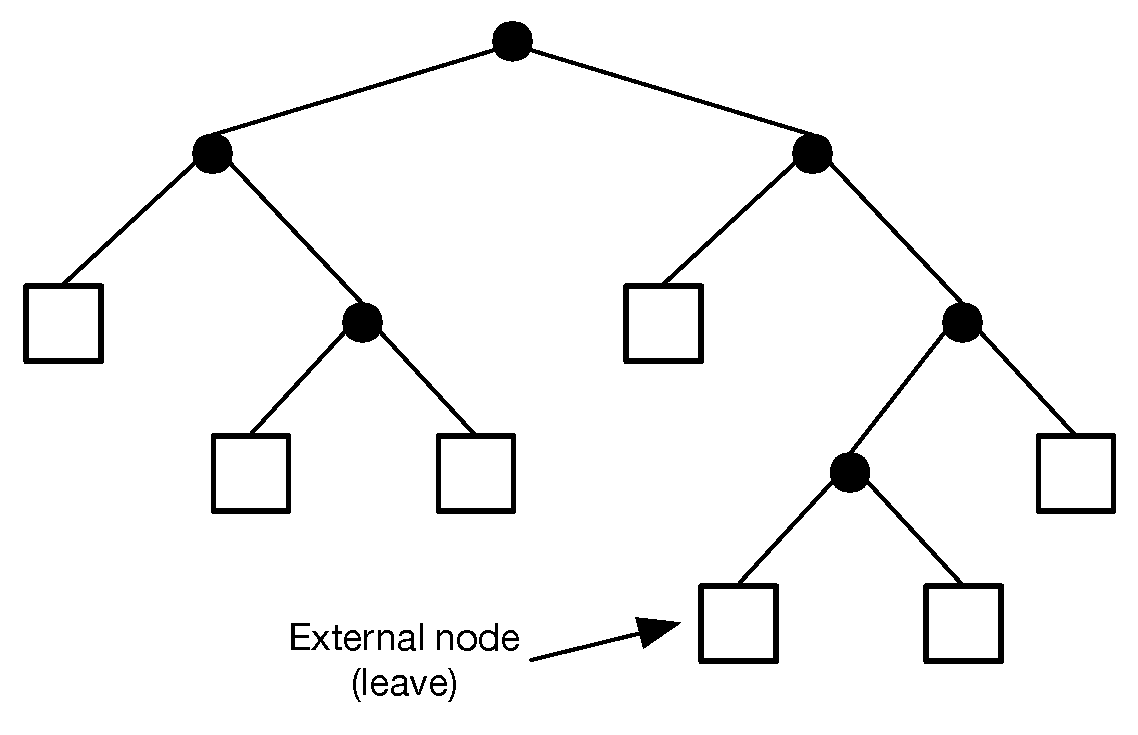
\includegraphics[width=0.7\textwidth]
      {02_higher_combinatorics/pics/BinaryTree}
  \caption{A binary tree}
\end{figure}

A binary tree is a plane structure.

\begin{center}
  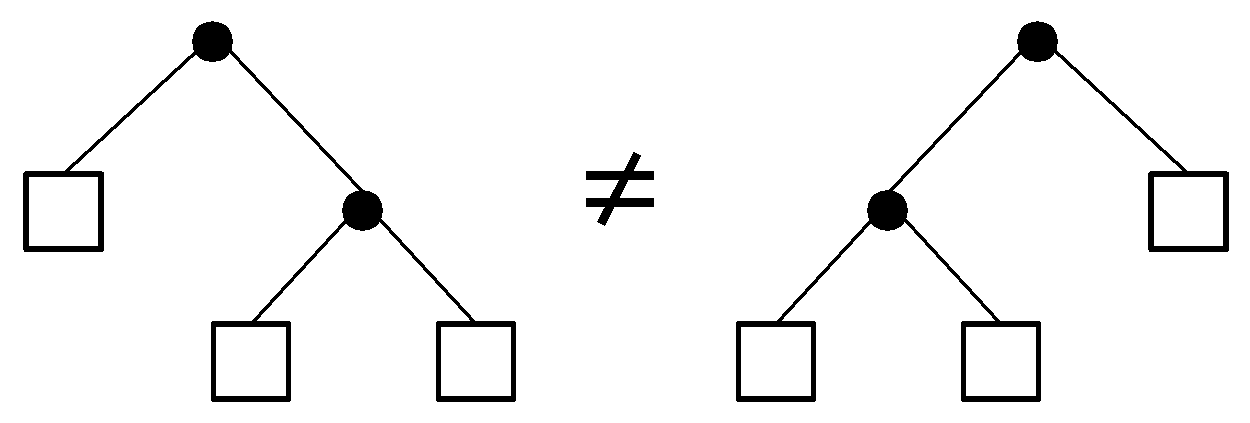
\includegraphics[width=0.7\textwidth]
    {02_higher_combinatorics/pics/BinaryTreeUnequal}
\end{center}

$a_n$ = number of binary trees with $n$ internal nodes

If there are n internal nodes, then there are n+1 leaves. The number of vertices in a binary tree is always odd ($n + (n+1)$). We try to describe the binary tree recursively.

\begin{center}
  Binary tree with size $n+1$ ($k$ ranges from $0$ to $n$):
  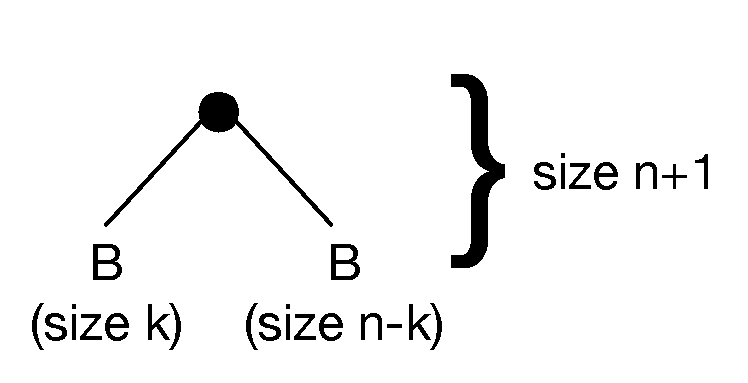
\includegraphics[width=0.5\textwidth]
    {02_higher_combinatorics/pics/BinaryTreeRecursion}
\end{center}
\begin{itemize}
  \item The left child has size $k$
  \item The right child has size $n-k$
\end{itemize}
\begin{align*}
    a_0 &= 1 \\
    a_{n+1} &= \sum_{k=0}^{n} a_k a_{n-k}
        \quad | \cdot z^{n+1} | \sum \\
    A(z) - 1 &= z A(z)^2
        \quad \text{(Cauchy-Product)} \\
    A(z) &= \frac{1 \pm \sqrt{1-4z}}{2z}\\
        &= \frac{1 \pm (1-4z)^\frac1{2}}{2z} \qquad
    \text{“$+$” is not a viable option, so we use “$-$”} \\
     \\
    (1 + z)^\alpha &= \sum_n {\binom{\alpha}{ n}} z^n \\
    (1-4z)^\frac1{2} &= \sum_{n \geq 0} \binom{\frac12}{n} \cdot (-4)^n \cdot z^n\\
	&= - \sum_{n\geq 0} \frac{\frac12 (-\frac12) (-\frac32) \ldots (\frac12 - n+1))}{n!} \cdot (-4)^n z^n \\
    &\sum_{n\geq 0} \underbrace{\frac{1}{n+1} {\binom{2n}{n}}}_{\text{ Catalan numbers}} z^n
\end{align*}
